\chapter{Positivity Bounds for Massive Scalars}
\label{chap:scalar}

In this chapter, we investigate positivity bounds on the spectrum of theories containing a massive scalar field. Our main goal is to understand how the allowed spectral region changes under different assumptions about the high-energy behaviour of the scattering amplitude.  

For the standard asymptotic behaviour implied by the Froissart bound,
\begin{equation*}
    \lim_{s \to \infty}\left|\frac{\mathcal{M}(s)}{s^{2}}\right|=0,
\end{equation*}
no restrictions on the spectrum arise.  

Then, we turn to theories satisfying the stronger condition
\begin{equation*}
    \lim_{s \to \infty}\left|s^{2}\mathcal{M}(s)\right|=0,
\end{equation*}
for which the amplitude obeys $-2$-th subtracted dispersion relations. In this case, we derive constraints on the spectrum by exploiting the positivity of the arc contributions.  

Finally, we study the intermediate scenario
\begin{equation*}
    \lim_{s \to \infty}\left|\mathcal{M}(s)\right|=0,
\end{equation*}
corresponding to $0$-th subtracted dispersion relations. For this setup, we obtain both analytical and numerical bounds on the spectrum using a general framework.

\section{$-2$-th Substracted Dispersion Relations}
To start, we will consider the 2 to 2 scattering of massless scalar particles with the exchange of a spin 0 resonance with mass $M$. The scattering amplitude is thus given by
\begin{align}
    \mathcal{M}(s, t, u) &= - \alpha^2 \left( \frac{1}{s-M^2} + \frac{1}{t-M^2} + \frac{1}{u -M^2} \right) - \notag \\ &\quad - \lambda
     + g_2(s^2 + t^2 + u^2) + g_3 \, stu + g_4 (s^2 + t^2 + u^2)^2 + \cdots
\end{align}
Taking into account that $s+t+u =0$ and working in the forward limit, this amplitude becomes
\begin{equation}
    \mathcal{M}_f(s) = - \lambda - a^2 \left( - \frac{1}{M^2} + \frac{1}{-M^2 + s} + \frac{1}{-M^2 - s}  \right) + 2 g_2 s^2 + 4 g_4 s^4 + \cdots
\end{equation}
The -2 substracted arc is given by 
\begin{equation}
    a_{-2} = \oint \frac{ds}{\pi i s}s^2 \;\mathcal{M}_f(s) = \sum \text{Res} \left(s \mathcal{M}_f(s) \right) = -2 \alpha^2 M^2 < 0.
\end{equation}
On the other hand, deforming the contour we know that 
\begin{equation}
    a_{-2} = \frac{2}{\pi} \int_{\Lambda^2}^{\infty} ds \; s \; \Im(\mathcal{M}_f(s)) \geq 0.
\end{equation}
Therefore, we arrive at a contradiction: the residue calculation yields \( a_{-2} = - 2 \alpha^2 M^2 < 0 \), while the dispersive representation, which follows from unitarity and analyticity, requires \( a_{-2} \ge 0 \). This inconsistency implies that a theory of massless scalar particles satisfying the \(-2\)-th subtracted dispersion relation cannot include the exchange of a massive spin-0 resonance. 

In the general case of the exchange of a massive resonance of even spin $J$, the amplitude can be written as  
\begin{equation}
    \begin{aligned}
    \mathcal{M}(s,t,u) &= - \alpha^2 \Bigg[ 
    \frac{\mathcal{P}_J\left(1 + \frac{2 t}{s}\right)}{s - M^2} 
    + \frac{\mathcal{P}_J\left(1 + \frac{2 s}{t}\right)}{t - M^2} 
    + \frac{\mathcal{P}_J\left(1 + \frac{2 s}{u}\right)}{u - M^2} 
    \Bigg] \\
    &\quad - \lambda 
    + g_2 (s^2 + t^2 + u^2) 
    + g_3\, s t u 
    + g_4 (s^2 + t^2 + u^2)^2 
    + \cdots,
    \end{aligned}
\end{equation}
which in the forward limit becomes
\begin{equation}
    \mathcal{M}_f(s) = - \alpha^2 \left[- \frac{1}{M^2}+ \frac{1}{s - M^2} + \frac{(-1)^J}{-s - M^2} \right] 
    - \lambda + 2 g_2 s^2 + 4 g_4 s^4 + \cdots
\end{equation}
Thus, the same argument applies: the residue calculation of the $-2$-subtracted dispersion relation gives a negative contribution, while unitarity requires a non-negative result.

This shows that a theory of \textbf{massless scalars satisfying  
$-2$-subtracted dispersion relations cannot consistently include the exchange of a massive resonance of even spin}. The inconsistency arises from the forward-limit behavior of the amplitude, which leads to a contribution that is always negative, violating the positivity constraint.

In the case in which the external legs have mass $m$, we can work with the crossing symmetric variable $\hat{s} = s - 2m^2$. The $-2$th substracted arc now becomes 
\begin{equation}
    a_{-2} = 2\alpha^2(2m^2 - M^2).
\end{equation}
This will be positive as long as 
\begin{equation}
    m^2 \geq \frac{M^2}{2},
\end{equation}
this is, the setup will be consistent as long as the mass of the resonance is small enough. In particular, the case $m = M$ (when the mass of the resonance is the same as the mass of the outer legs) is consistent.

\section{0-th subtracted dispersion relations}

We now assume that the amplitude satisfies a 0-th subtracted dispersion relation. 
Applying the method described above does not immediately lead to bounds on the spectrum. 
Nevertheless, we will show that it is still possible to derive systematic constraints. 
Moreover, we will use the method introduced in \Cref{sec:res} to numerically strengthen the bounds obtained analytically.

In what follows, we consider $2 \to 2$ scattering of identical scalars, either massless or massive. 
Our goal is to investigate the allowed mass of a spin-2 resonance exchanged in the amplitude, in the presence of additional possible spin-0 resonances.

\subsection{Analytic Bounds on the Spectrum}

We will now describe the method presented in \autocite{Berman:2024kdh} to find analytic bounds on the spectrum. Consider again the $2 \to 2$ scattering of massless scalars, and define the arcs as 
\begin{equation}
    a_n^m = \frac{1}{m!} \partial_t^m \Big|_{t = 0} 
    \sum_{J=0}^{\infty} \frac{1}{s^n} 
    \mathcal{P}_J \left( 1 + \frac{2t}{s} \right) 
    \rho_J(s),
\end{equation}
where $\rho_J(s) \geq 0$ is the spectral density in the spin-$J$ channel. 

The setup will be the following: suppose we have a certain cutoff $\Lambda^2$. Bellow it, we will have a series of masses $m_1^2, m_2^2, \ldots$ We will only allow for resonances to apper at these masses. Our goal now is to study which is the highest possible spin, $J_1$, that can be exchanged at the lowest mass, $m_1$. 

Consider a resonance of spin $J$ and mass $m_n$. As discussed in \Cref{sec:res}, it contributes to the amplitude as 
\begin{equation}
    \mathcal{M}(s, t) \sim -  \lambda_{J,n}^2 
    \left( 
    \frac{\mathcal{P}_J \left( 1 + \frac{2t}{s} \right)}{s - m_n^2} 
    + 
    \frac{\mathcal{P}_J \left( 1 + \frac{2t}{u} \right)}{u - m_n^2} 
    \right).
\end{equation}
Since 
\begin{equation}
    \mathcal{P}_J(1 + x) \sim x^J,
\end{equation}
a spin-$J$ state generates contributions growing as $s^J$ at high energies. 
However, in order for the $0$-th subtracted dispersion relation to exist, the amplitude must not grow too fast at large $s$. Therefore, the contributions from high spins must combine in such a way that this growth cancels. As we now show, this requirement leads to non-trivial constraints on the spectrum.

The dispersion relation for the Wilson coefficients $a_{k,q}$ reads
\begin{equation}
    a_{k,q} \sim 
    \sum_{J=0}^{\infty} 
    \int_{m_1^2}^{\infty} ds 
    \frac{\rho_J(s)}{s^{k+1}} 
    v_{J,q},
\end{equation}
where $\rho_J(s) \geq 0$ and $v_{J,q} > 0$ arise from expanding the Legendre polynomials. 
Importantly, $v_{J,q} = 0$ for $q < J$.

Defining the dimensionless variable
\begin{equation}
    y = \frac{s}{m_1^2},
\end{equation}
and rescaling
\begin{equation}
    (m_1^2)^k a_{k,q} \to a_{k,q},
\end{equation}
the dispersion relation becomes
\begin{equation}
    a_{k,q} =
    \sum_{J=q}^{\infty} 
    \int_{1}^{\infty} dy \, 
    f_J(y) \, y^{-k} \, v_{J,q},
\end{equation}
with $f_J(y)\geq 0$.


We introduce the dimensionless squared masses
\begin{equation}
    \mu_n = \frac{m_n^2}{m_1^2},
\end{equation}
and define the bracket
\begin{equation}
    \langle y^{-k} v_{J,q} \rangle_{\mu_n}
    =
    \sum_{J=q}^{\infty} 
    \int_{\mu_n}^{\infty} dy \,
    f_J(y) \, y^{-k} \, v_{J,q}.
\end{equation}
Then,
\begin{equation}
    a_{k,q} = \langle y^{-k} v_{J,q} \rangle_{1}.
\end{equation}

Assume the theory is weakly coupled and possesses a mass gap: the first states appear at $m_1^2$, and the next threshold is at $m_2^2 > m_1^2$. 
Let $J_1$ denote the highest spin present at the first mass level. Then
\begin{equation}
    a_{k,q} =
    \sum_{J=q}^{J_1} 
    \lambda_{J,1}^2 v_{J,q}
    +
    \langle y^{-k} v_{J,q} \rangle_{\mu_2}.
\end{equation}

Since $\mu_2>1$, the right-hand side vanishes as $k \to \infty$, and thus
\begin{equation}
    \lim_{k \to \infty} a_{k,J_1}
    =
    \lambda_{J_1,1}^2 v_{J_1,J_1}.
\end{equation}
We have isolated a Wilson coefficient that depends only on the coupling of the highest-spin state at the mass gap.

For $k \geq J_1$ we have
\begin{equation}
    y^{-k}
    =
    \mu_2^{-k}
    \left( \frac{y}{\mu_2} \right)^{-k}
    \leq
    \mu_2^{-k}
    \left( \frac{y}{\mu_2} \right)^{-J_1}.
\end{equation}
Therefore,
\begin{equation}
    \langle y^{-k} v_{J,J_1} \rangle_{\mu_2}
    \leq
    \frac{1}{\mu_2^{k-J_1}}
    \langle y^{-J_1} v_{J,J_1} \rangle_{\mu_2}.
\end{equation}

Crossing symmetry implies
\begin{equation}
    a_{k,k-J_1} = a_{k,J_1}.
\end{equation}
Moreover, as shown in \autocite{Berman:2024kdh}, positivity of the dispersive representation implies the inequality 
\begin{equation}
    \left( \frac{a_{k,q}}{a_{q,q}} \right)^{\frac{k'-q}{k-q}}
    \leq
    \left( \frac{a_{k',q}}{a_{q,q}} \right).
\end{equation}
Taking $q = k - J_1$ and $k' = k+1$, we obtain
\begin{equation}
    \left( 
    \frac{a_{k,k-J_1}}{a_{k-J_1,k-J_1}} 
    \right)^{1 + 1/J_1}
    \leq
    \frac{a_{k+1,k-J_1}}{a_{k-J_1,k-J_1}}.
\end{equation}

Using crossing again,
\begin{equation}
    a_{k+1,k-J_1} = a_{k+1,J_1+1}.
\end{equation}
Since $v_{J_1,J_1+1}=0$, the first mass level does not contribute to this coefficient, and therefore
\begin{equation}
    a_{k+1,J_1+1}
    =
    \langle y^{-(k+1)} v_{J,J_1+1} \rangle_{\mu_2}.
\end{equation}
As $k \to \infty$, this vanishes.

On the other hand,
\begin{equation}
    \lim_{k \to \infty} a_{k-J_1,0}
    =
    \sum_{J=0}^{J_1} 
    \lambda_{J,1}^2 v_{J,0}.
\end{equation}

Taking the large-$k$ limit of the inequality, we obtain
\begin{equation}
    \left(
    \frac{\lambda_{J_1,1}^2 v_{J_1,J_1}}
    {\sum_{J=0}^{J_1} \lambda_{J,1}^2 v_{J,0}}
    \right)^{1 + 1/J_1}
    \leq 0.
\end{equation}
Since the right-hand side vanishes and the left-hand side is positive, we conclude that
\begin{equation}
    \lambda_{J_1,1}^2 = 0.
\end{equation}

We therefore find that no state with spin $J_1 \geq 1$ can sit at the mass gap. The only allowed spin for a resonance at $s = m_1^2$ is $J = 0$.

It is important to stress why the argument does not apply to the case $J_1 = 0$. 
The derivation of the inequality relied on choosing 
\begin{equation}
    q = k - J_1,
\end{equation}
which ensures that the coefficient $a_{k,k-J_1}$ isolates the highest spin contribution at large $k$. 
However, when $J_1 = 0$, this choice gives $q = k$, and therefore the inequality becomes
\begin{equation}
    \left( \frac{a_{k,k}}{a_{k,k}} \right)^{1 + 1/0}
    \leq
    \frac{a_{k+1,k}}{a_{k,k}}.
\end{equation}
This expression is ill-defined, since the exponent diverges for $J_1 = 0$. 
More importantly, crossing symmetry implies in this case
\begin{equation}
    a_{k+1,k} = 0,
\end{equation}
because $v_{0,1}=0$ and there is no contribution from the first mass level to this coefficient. 
Therefore the Hankel inequality is trivially satisfied and does not impose any constraint on $\lambda_{0,1}^2$.

What we have found is that there can only be exchange of a spin 2 resonance of mass $m_2$ if there is exchange of a scalar resonance of mass $m_1 < m_2$. If there is no exchange of a scalar particle, the higher spin particle can not be exchanged.

A similar argument applies to the $2 \to 2$ scattering of massive scalars. 
The main difference is that the location of the resonances is shifted by the external mass. 
In this case, the first resonance appears at 
\[
\lvert m_1^2 - 2m^2 \rvert,
\]
and the second at 
\[
\lvert m_2^2 - 2m^2 \rvert.
\]

The situation becomes particularly interesting if the scalar that is being exchanged is the same particle as the one being scattered. 
Then the first resonance occurs at
\[
\hat{s} = m^2,
\]
while the second remains at
\[
\hat{s} = \lvert m_2^2 - 2m^2 \rvert.
\]

We therefore conclude that the exchange of a spin-2 ($J=2$) particle of mass $m_2$ is possible only if
\[
\lvert m_2^2 - 2m^2 \rvert \geq m^2 \Rightarrow m_2^2 \geq 3m_0^2 \text{ or } m_2^2 \leq m^2.
\]


\subsection{Numerical Bounds on the Spectrum}
Now we are going to use the method described in \Cref{sec:res} to numerically find the maximum value of 
$$
\frac{\lambda_j^2}{m_j^2 g_0},
$$
where $\lambda_j^2$ is the coupling of the spin $j$ resonance to the scalar, $m_j$ its mass and $g_0$ the 4-point coupling.

We start by considering \textbf{massless external legs, and the exchange of a spin 0 resonance}. The higher bound for 
$$
\frac{\lambda_0^2}{m_0^2 g_0}
$$
is shown in \Cref*{fig:scalar_comparison}. The drop at low masses is a numerical artifact, arising from the limited number of partial-wave contributions included in the computation, as we can see from adding high $J$ terms such as $10^5 J_{\text{max}}$. Therefore, this configuration of massless external scalars and a massive spin-0 resonance is consistent for any value of the resonance mass. This is compatible with the analytic results previously mentioned: we found no bounds on the mass of a single scalar resonance.

\begin{figure}[hbtp]
    \centering
    \begin{subfigure}[t]{0.48\textwidth}
        \centering
        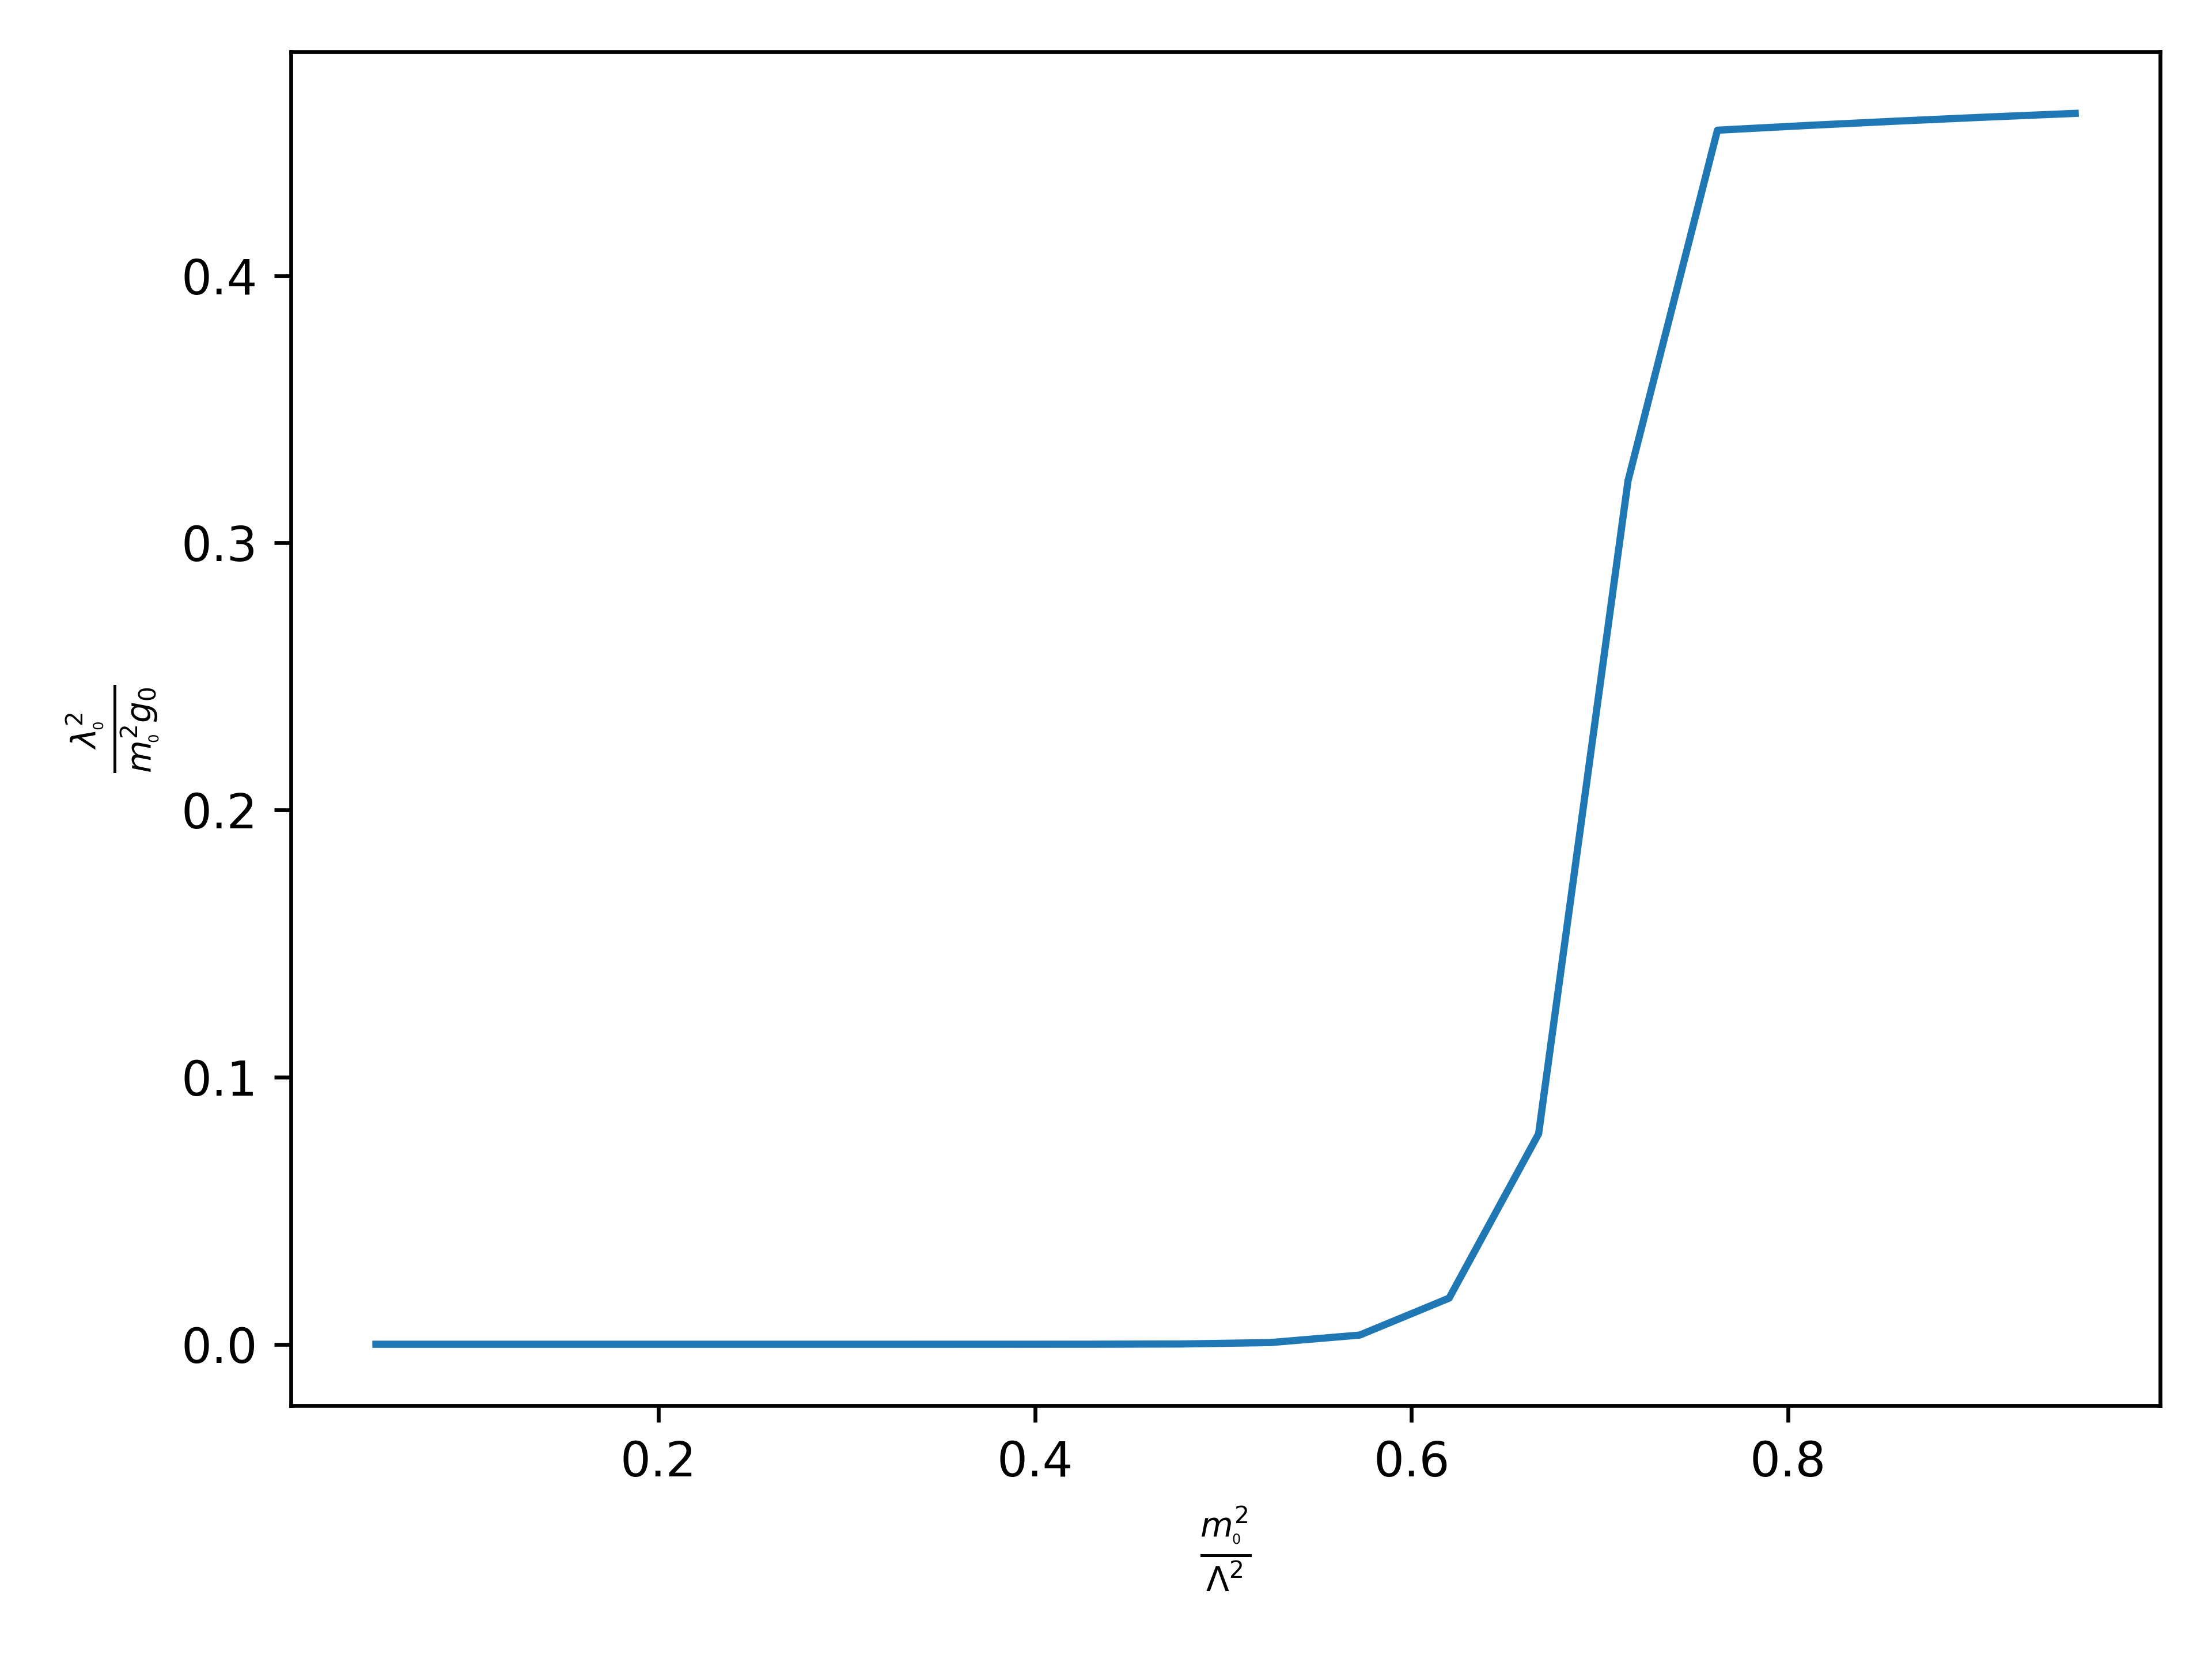
\includegraphics[width=\textwidth]{figures/scalar_scalar.png}
        \caption{Without higher-order terms}
        \label{fig:scalar_scalar}
    \end{subfigure}
    \hfill
    \begin{subfigure}[t]{0.48\textwidth}
        \centering
        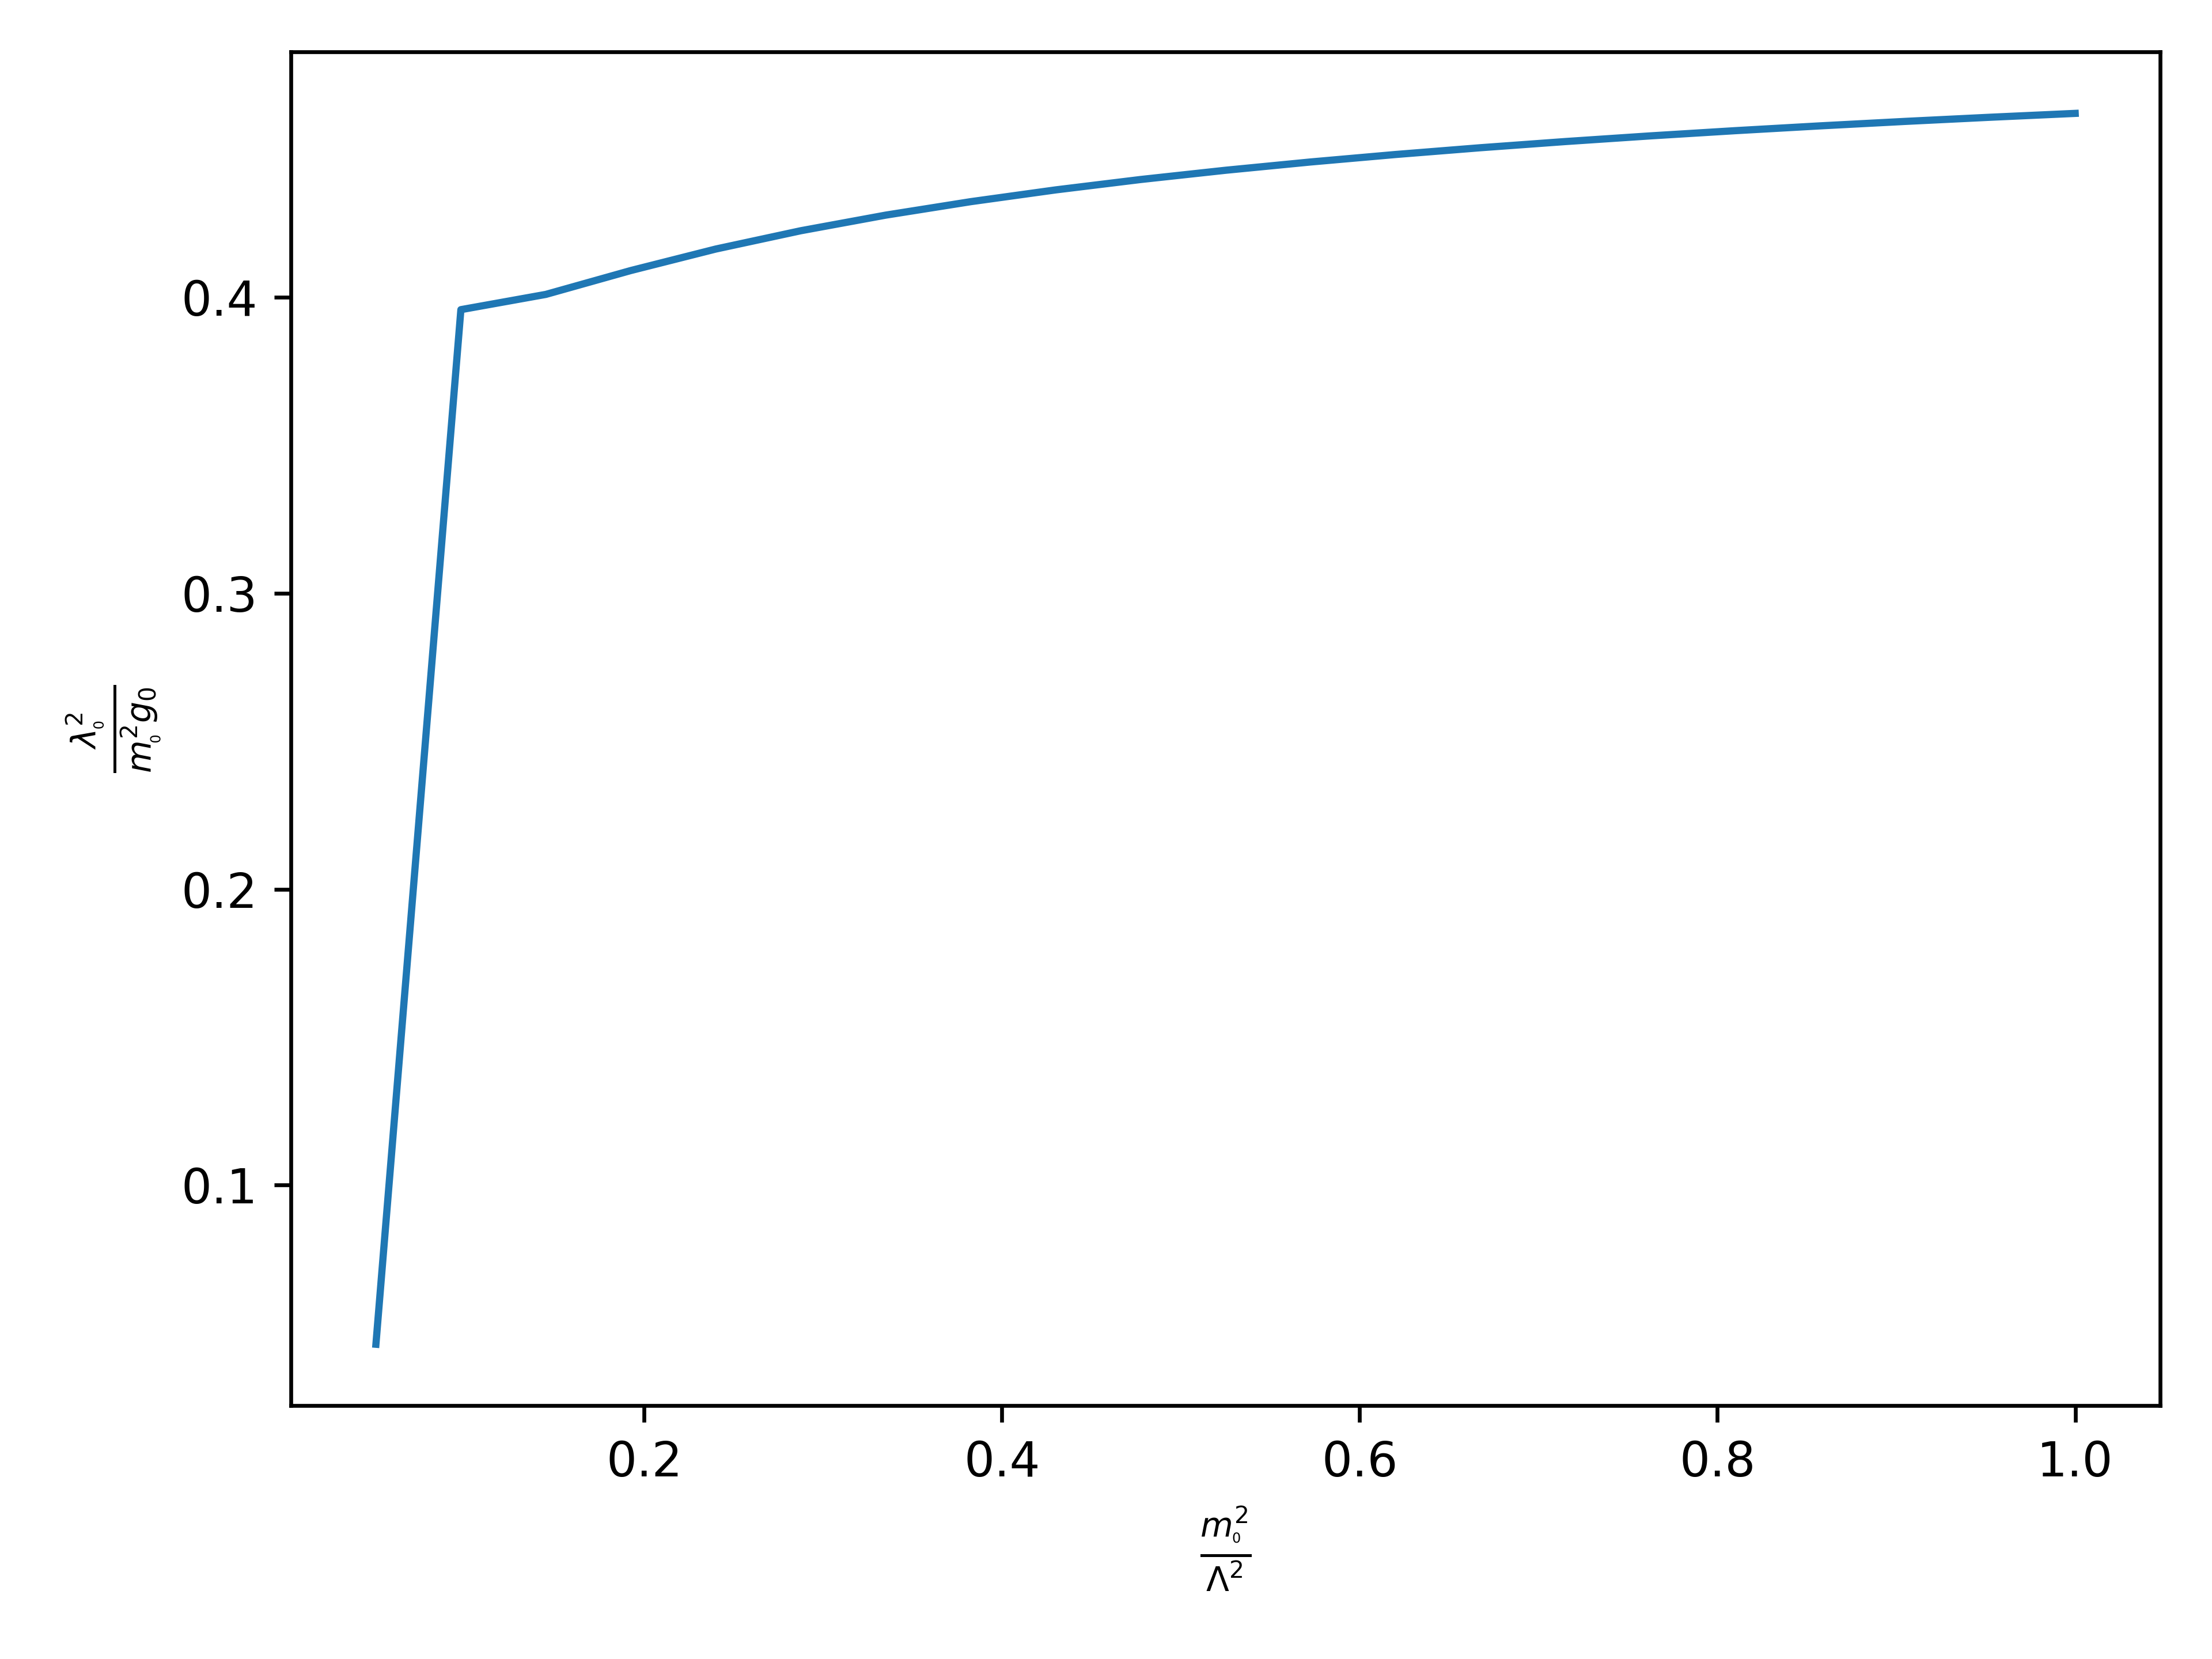
\includegraphics[width=\textwidth]{figures/scalar_scalar_with_high.png}
        \caption{Including higher-order terms}
        \label{fig:scalar_scalar_with_high}
    \end{subfigure}
    \caption{Comparison of the scalar-scalar scattering amplitude with $J_{max}=100$ and with $J_{max} = 100 \cdot 10^4$.}
    \label{fig:scalar_comparison}
\end{figure}

Then, we consider \textbf{massless external legs, and the exchange of a spin 2 resonance}. The results are shown in \Cref*{fig:massless_spin2}. The tail is a numerical artifact: in this setup, we obtain that the spin-2 particle must lie above the cutoff. This result remains stable for all values of $J_{\text{max}}$. This is again compatible with the analytical results found before: a spin 2 resonance can not be exchanged if there is not a spin 0 resonance at a lower mass.

\begin{figure}[hbtp]
    \centering 
    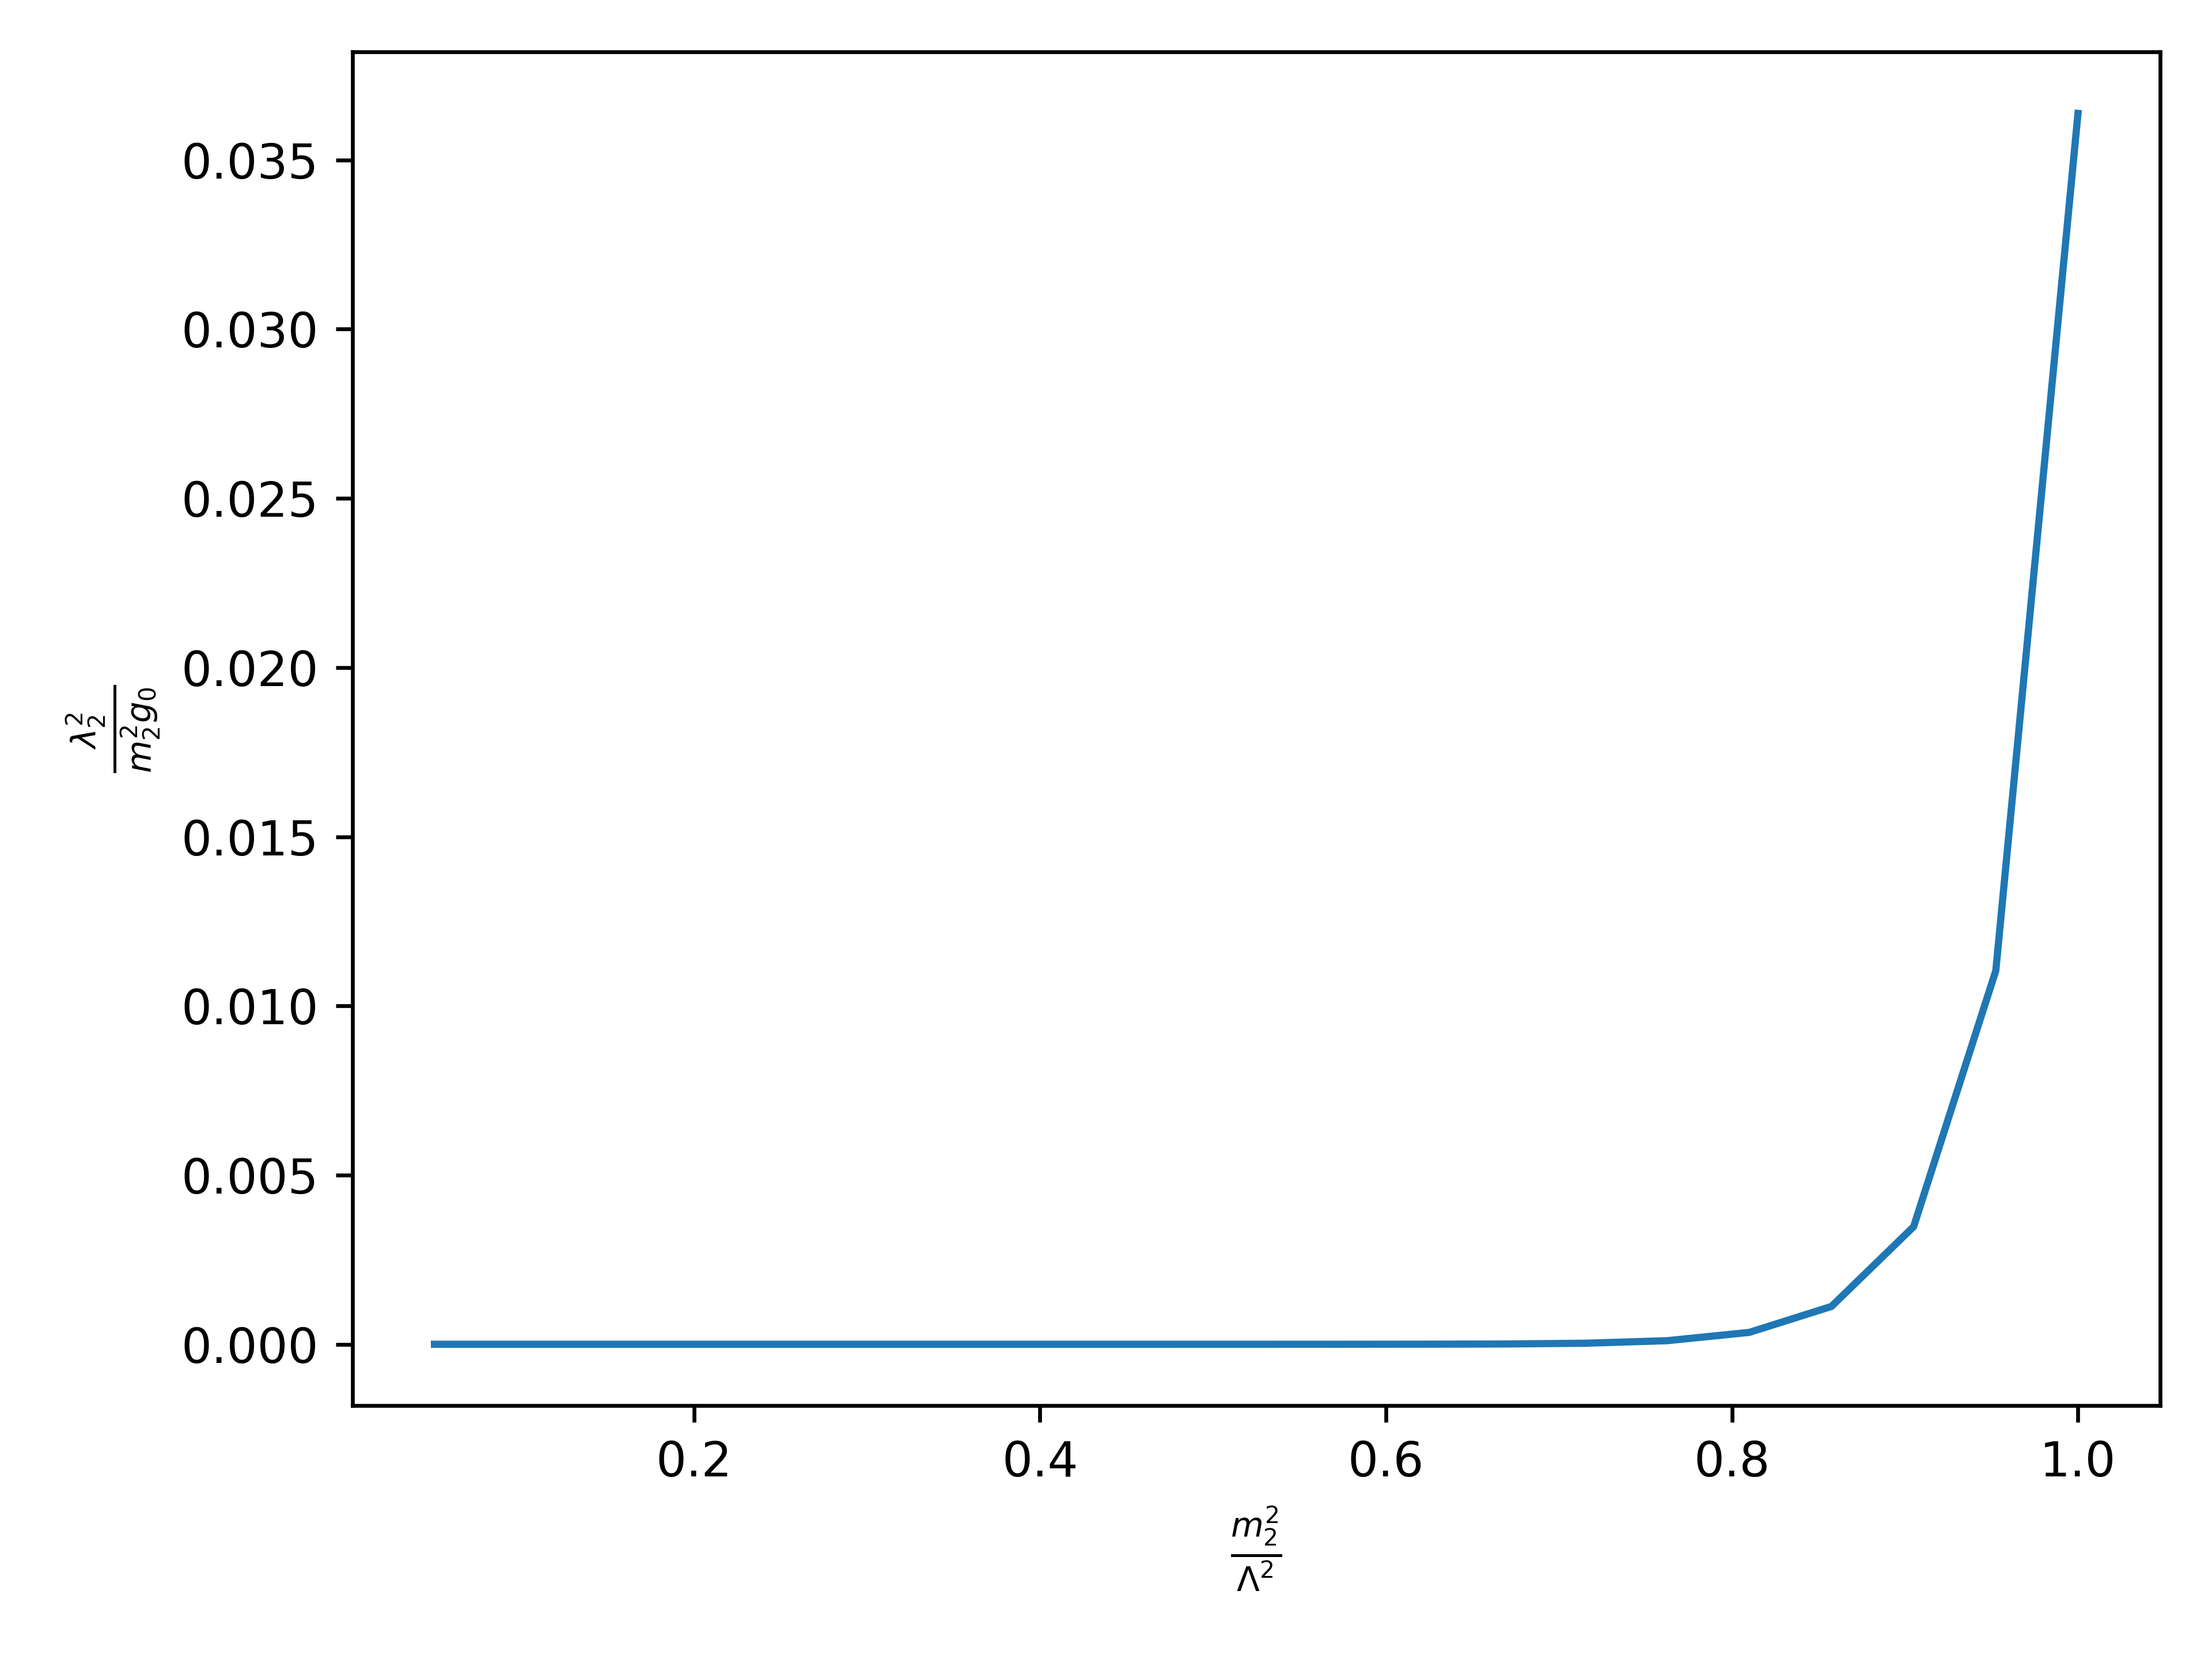
\includegraphics[width = 0.75\textwidth]{figures/plot.png}
    \caption{Bounds for a massive spin 2 resonance and massless external legs.}
    \label{fig:massless_spin2}
\end{figure}

Next, we consider the case of \textbf{massive external legs with the exchange of a spin-2 resonance}, shown in \Cref*{fig:massive_scalar_spin_2}. As in the previous scenario, the appearance of tails is a numerical artifact. This indicates, once again, that the resonance lies above the cutoff, so this scenario is not consistent, and is compatible with the analytical result.
\begin{figure}[hbtp]
    \centering
    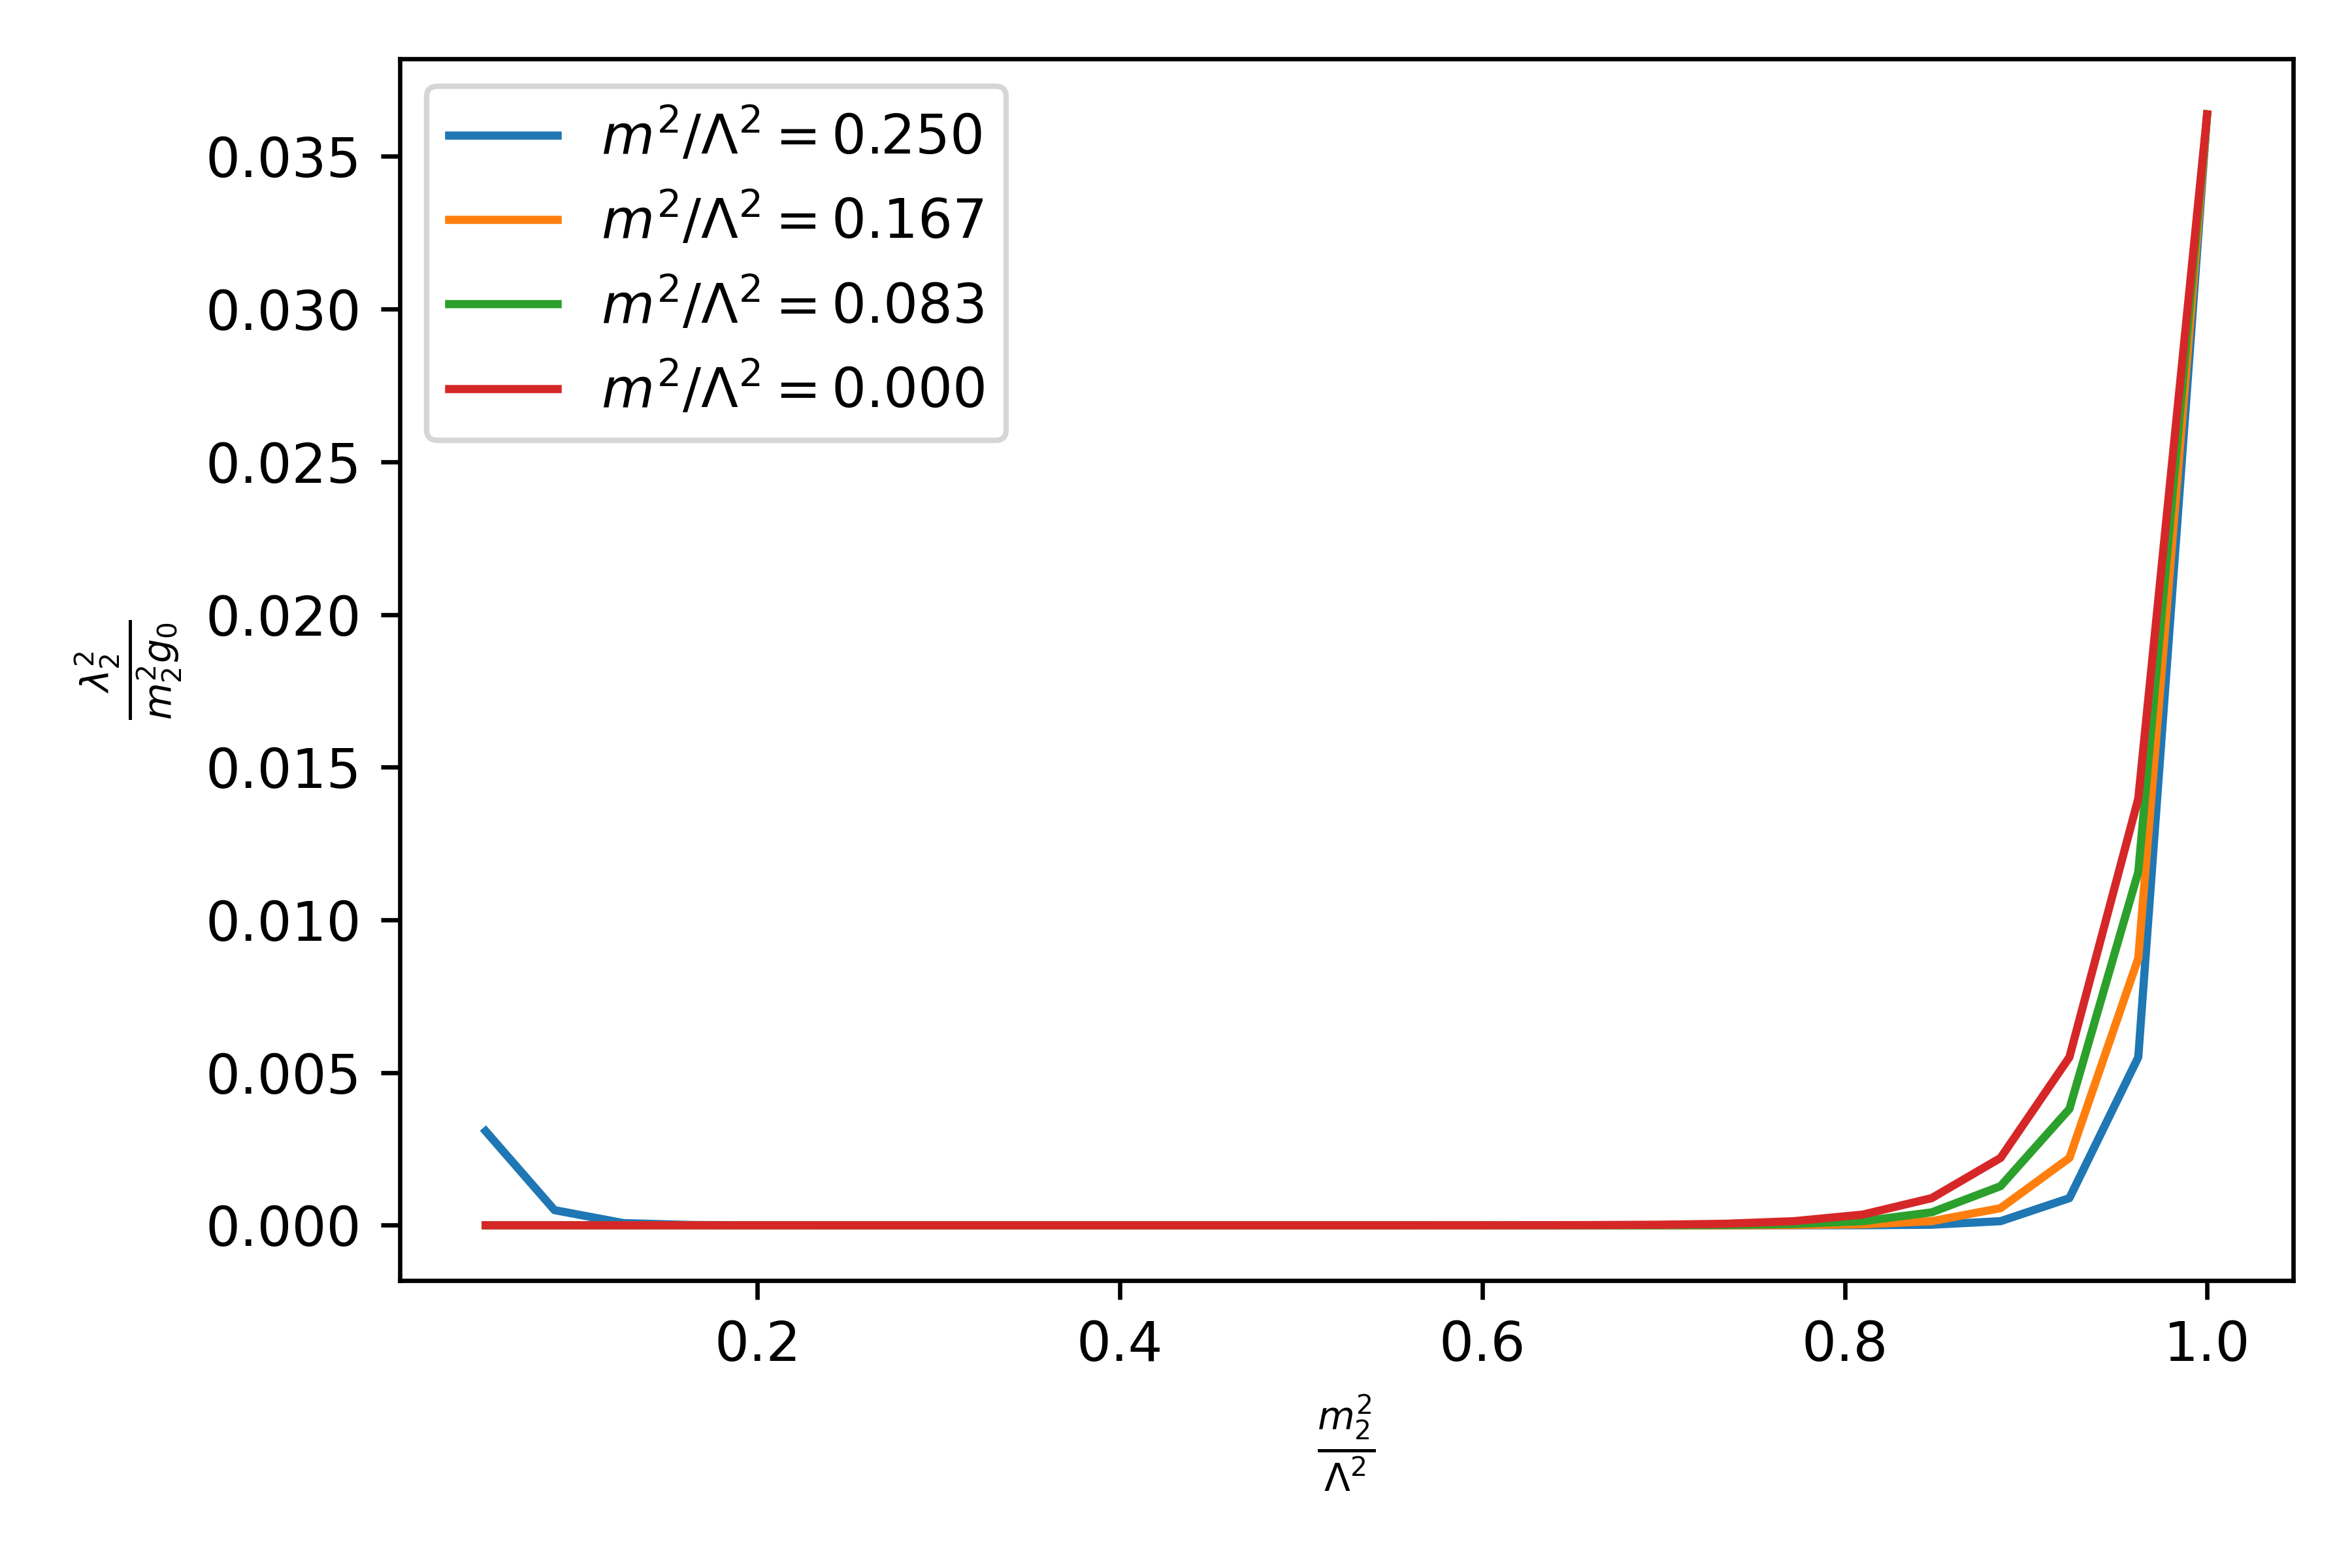
\includegraphics[width = 0.75\textwidth]{figures/bounds_corrected2.png}   
    \caption{Bounds for a massive spin 2 resonance and massive scalar external legs.} 
    \label{fig:massive_scalar_spin_2}
\end{figure}

So far, we have established that it is not possible to construct a consistent theory for a scalar field exchanging only a spin-2 particle below the cutoff while satisfying unsubtracted dispersion relations. We now turn to more complex scenarios.
As a first step, we consider \textbf{massless external legs with the exchange of both spin-2 and spin-0 resonances}. The corresponding bounds, for different values of the spin-0 mass, are shown in \Cref*{fig:massive_scalar_spin_23}. As can be seen, the theory becomes consistent when the mass of the spin-2 resonance approaches the cutoff. Analytically, we know that 
$$
m_2^2 > m_0^2.
$$
The numerical results presented here provide a stronger version of this bound.
\begin{figure}[hbtp]
    \centering
    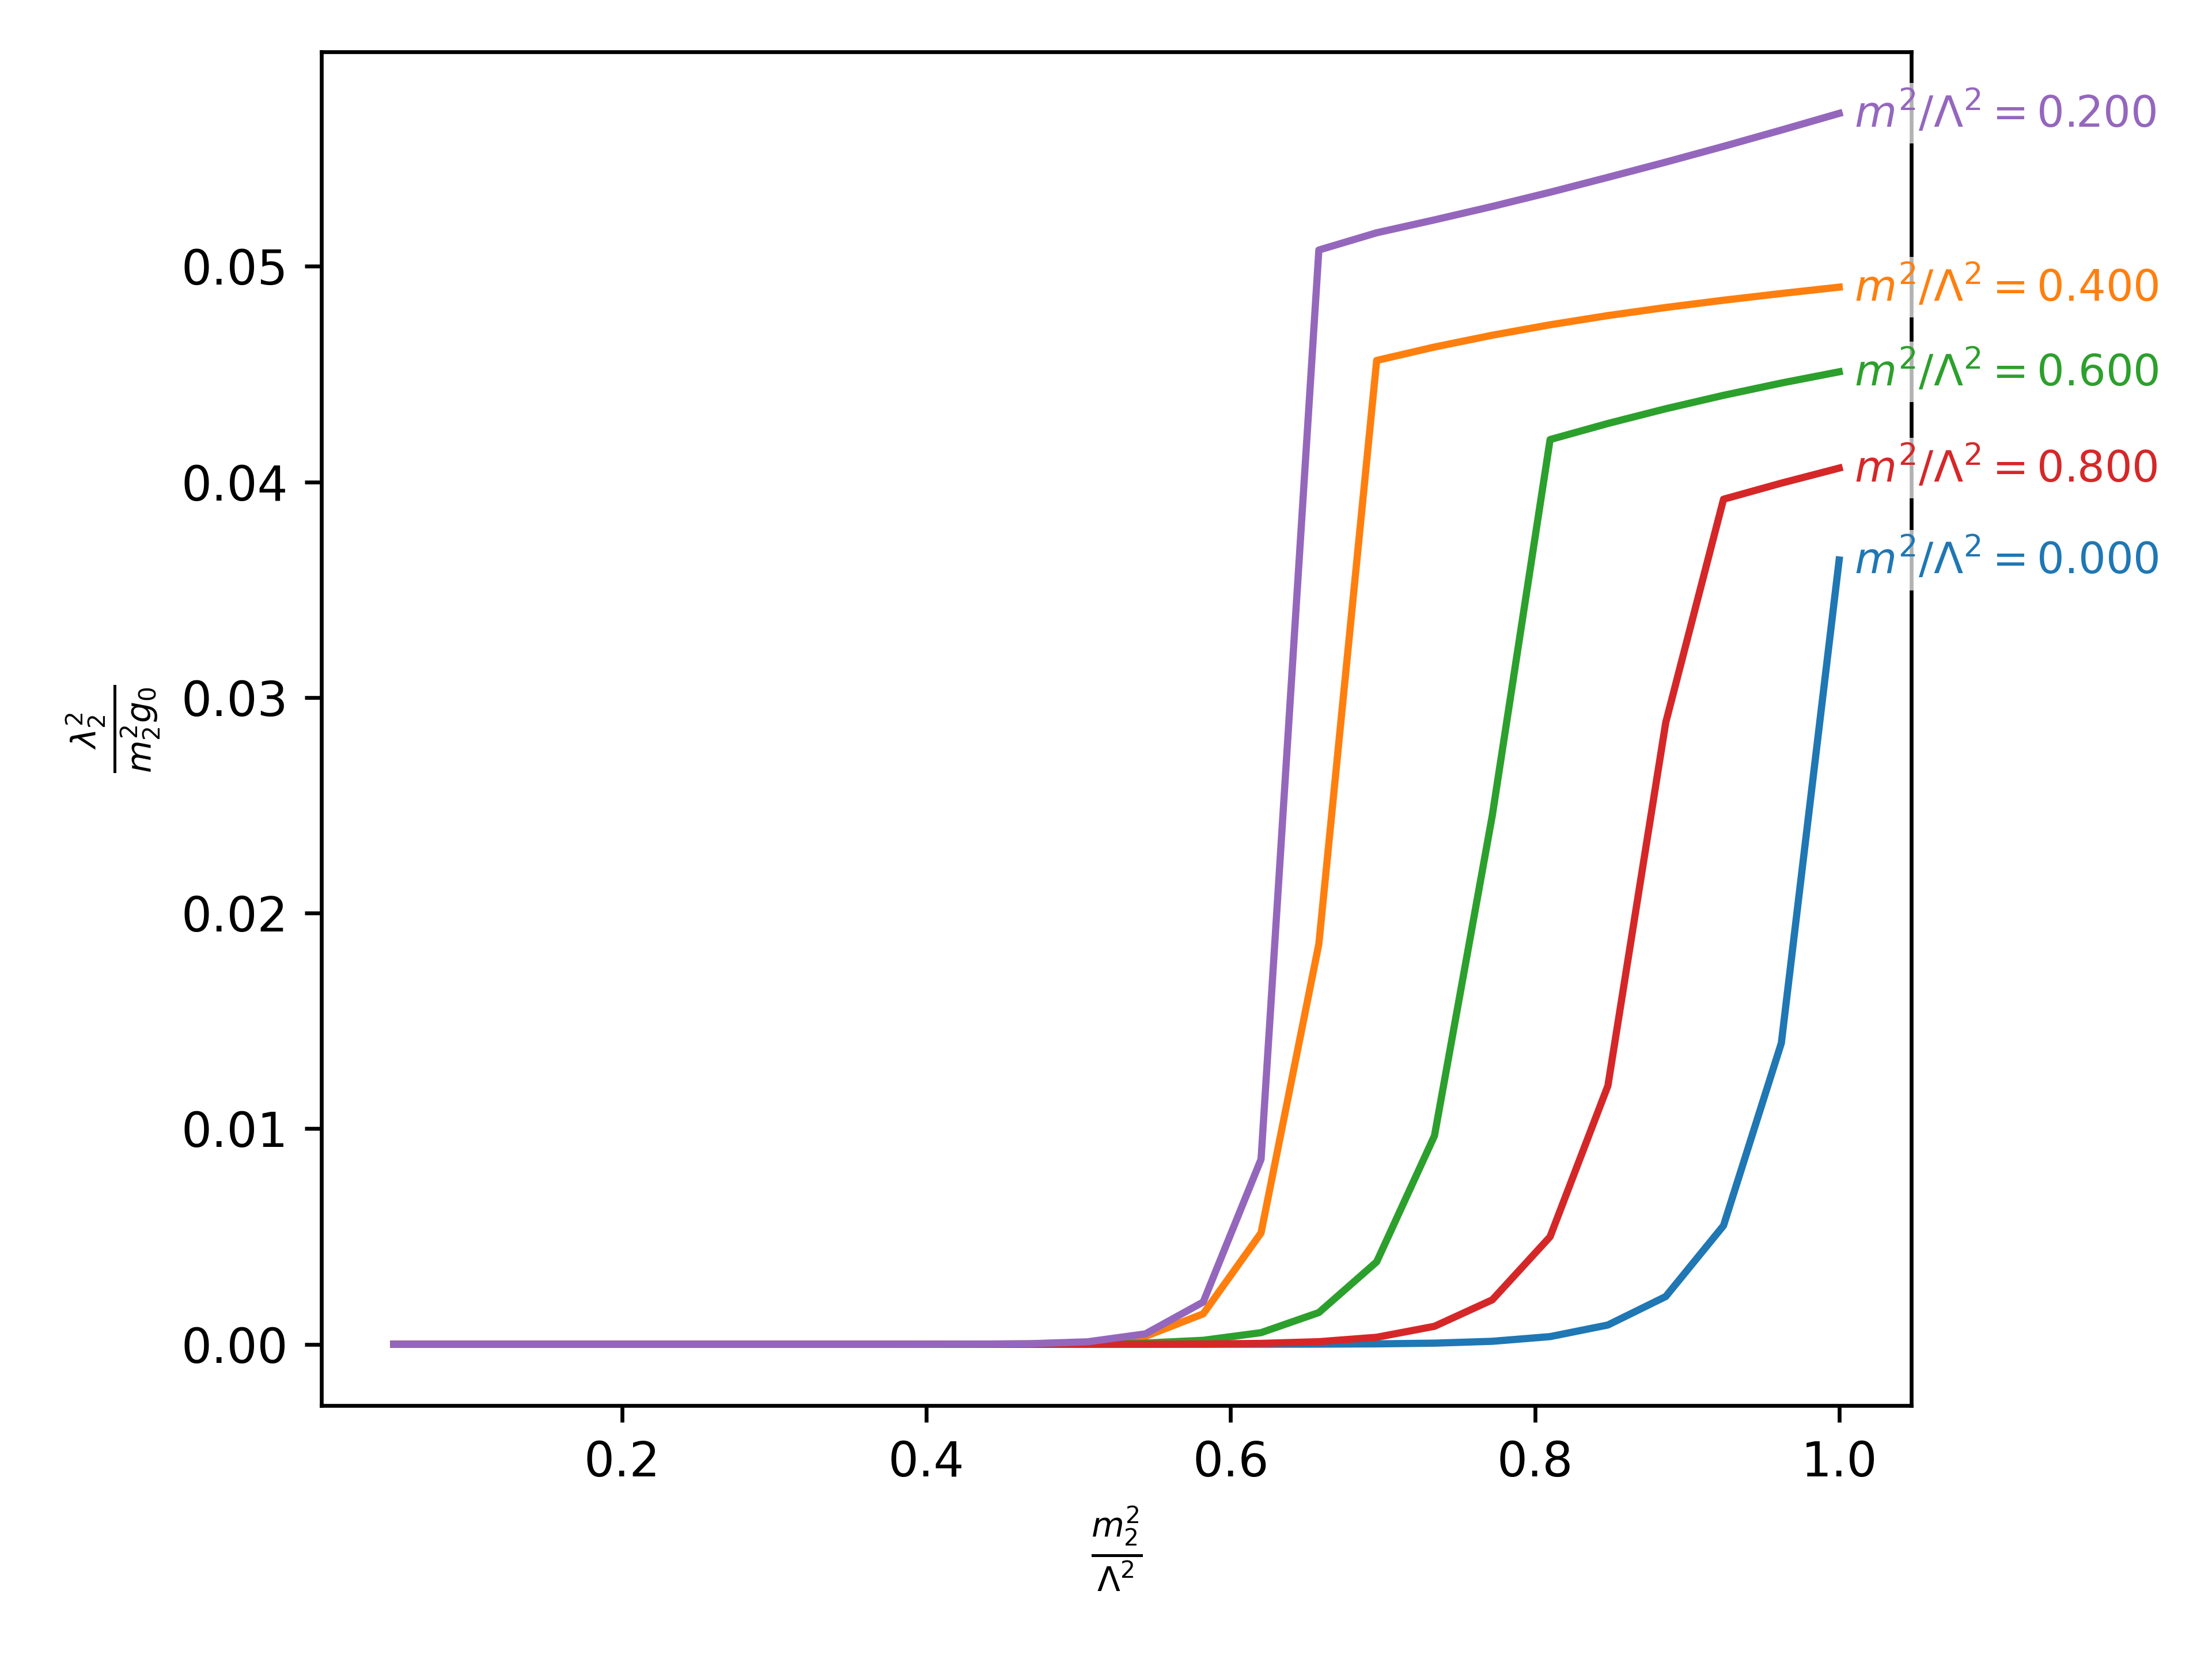
\includegraphics[width = 0.75\textwidth]{figures/two_res.png}
    \caption{Bounds for a massive spin 2 resonance and a massive spin 0 resonance with massless scalar external legs, shown for different values of the spin 0 mass. The blue line represents the bound in the absence of spin 0 exchange.}
    \label{fig:massive_scalar_spin_23}
\end{figure}

Finally, we explore the case of \textbf{massive external legs with the exchange of both spin-2 and spin-0 resonances}, where the mass of the spin-0 resonance is taken to be equal to that of the external legs.
The bounds are shown in figure \Cref*{fig:2res}. Analytically,
$$
\abs{m_2^2 - 2m_0^2} > m_0^2,
$$
which defines two regions in which we expect to find consistent theories:
$$
m_2^2 > 3m_0^2 \;\text{ and }  \; m_2^2 < m_0^2.
$$
These features are also reproduced in the numerical results, and are particularly evident for $m_0^2 = 0.25,\Lambda^2$. Once again, the numerical analysis gives a stronger version of the analytical bound.
\begin{figure}[hbtp]
\centering
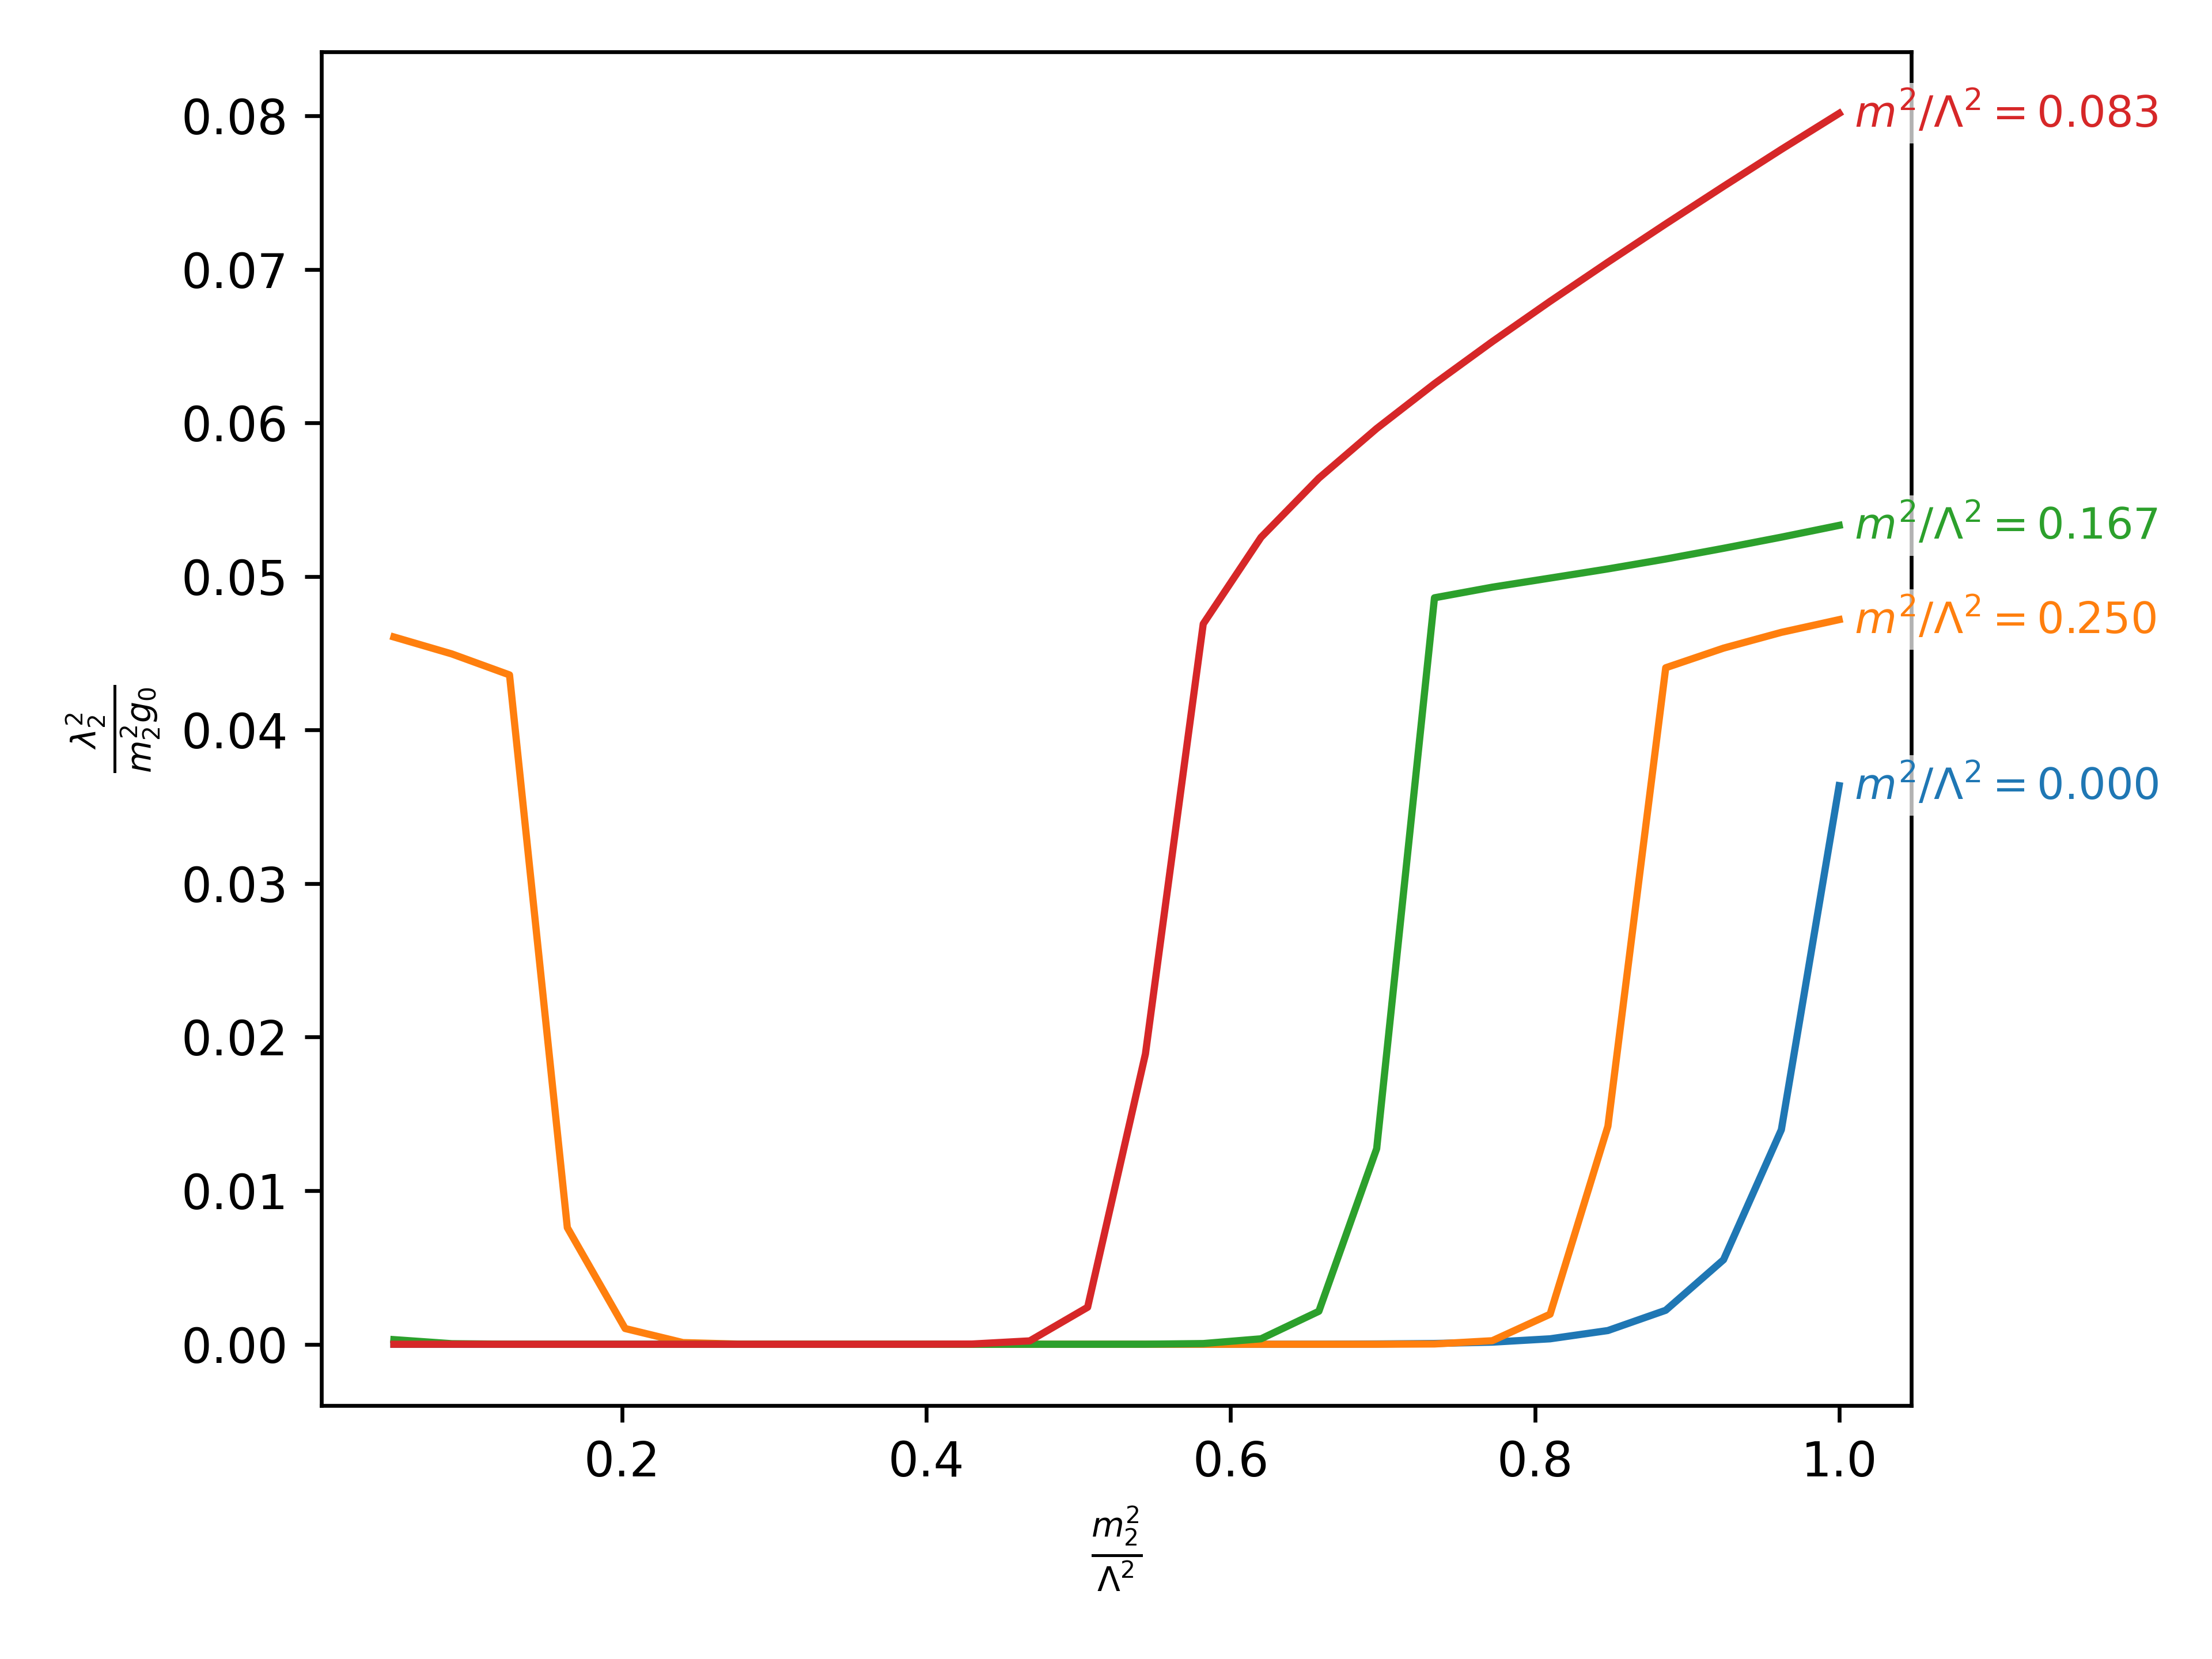
\includegraphics[width = 0.75\textwidth]{figures/new_bounds.png}
\caption{Bounds for a massive spin 2  resonance and a massive spin 0 resonance with massive scalar external legs, shown for different values of the external mass. The spin 0 resonance and the external legs have equal mass. The blue line represents the bound in the absence of spin 0 exchange.}
\label{fig:2res}
\end{figure}